% Лекции Сергея Борисовича Стечкина
% Внесены исправления В.В.Арестова, версия 06.07.2009
% Внесены исправления Н.И.Черныха, версия 24.07.2009
% Внесена грамматическая и ТеХ-правка М.Дейкаловой, версия 05.08.09

%%%%%%%%%%%%%%%%%%%%%%%%%%%%%
\chapter{Неравенство Колмогорова.\\
Приближение гладкими функциями.\\ Функция Стеклова.\\
Неравенство Джексона}
%%%        Лекция 20.

\section{Второе доказательство неравенства Колмогорова в $C_{2\pi}$}


 В конце прошлой лекции было доказано неравенство Колмогорова между нормами
 производных дифференцируемых периодических функций, а точнее, было доказано
 следующее утверждение.

 {\it При любых $0<k<n$ существуют константы $K_{n,k}$ такие, что
  \begin{equation}\label{f20-1}
 \|f^{(k)}\|_C\le K_{n,k}\|f\|^{\frac{n-k}{n}}_C\cdot
 \|f^{(n)}\|^{\frac{k}{n}}_C,\qquad f\in C^{(n)}_{{2\pi}}.
 \end{equation}
 }

 При $k=0$ и $k=n$ неравенство~(\ref{f20-1}), очевидно, {также}
 выполняется {с} {константой $1$}.

 Выведем неравенство~(\ref{f20-1}) из обобщенного неравенства
 Бернштейна~(\ref{f19-6}).  Заменим  параметр $n$ на параметр  $l.$ Пусть     $0<k<l.$
 Для функции  $f\in C^{(k)}_{{2\pi}}$
 по обобщенному неравенству Бернштейна (теорема~\ref{t-o-bern})
  \begin{equation}\label{f20-2}
 \|f^{(k)}\|_C\le n^k \|f\|_C+A_kE_n(f^{(k)})_C.
 %\eqno(1)
  \end{equation}
 Это неравенство было доказано только для натуральных $n,$
 но так как $f^{(k)}\perp \mbox{const},$ то оно верно и для  $n=0.$
 Применим к $f^{(k)}$ неравенство Фавара~(\ref{f19-4}):
 $$
 E_n(f^{(k)})_C\le \frac{M_{l-k}}{(n+1)^{l-k}}\|f^{(l)}\|_C,
 $$
где $M_{l-k}$ -- константы Фавара, для которых, как было
отмечено ранее, справедлива оценка $M_{l-k}\le \dfrac{\pi}{2}.$
 Тогда из~(\ref{f20-2}) получим
 \begin{equation}\label{f20-3}
 \|f^{(k)}\|_C\le
 n^k\|f\|_C+C_k'\frac{\|f^{(l)}\|_C}{(n+1)^{l-k}}\qquad \forall\
 n=0,1,\ldots
 \end{equation}
 Для вещественного параметра $h>0$ выберем целое неотрицательное число $n$  по правилу
 $\dfrac{1}{n+1}<
 h\le \dfrac{1}{n}$ при $0<h\le 1$ и $n=0$ при $h>1.$
 Тогда из~(\ref{f20-3}) следует  неравенство
 $$
 \|f^{(k)}\|_C\le h^{-k}\|f\|_C+C_k' h^{l-k}\|f^{(l)}\|\qquad \forall\
 h>0
 $$
 или
 \begin{equation}\label{f20-4}
 \|f^{(k)}\|_C\le C_k (h^{-k}\|f\|_C+h^{l-k}\|f^{(l)}\|_C)\qquad
 \forall\ h>0,
 \end{equation}
 где $C_k=\max\{1,C_k'\}.$
 Выберем параметр $h$ так, чтобы правая часть последнего  неравенства  имела  наименьшее,
 или близкое к наименьшему,  значение.

 В таких ситуациях оказывается полезным следующий принцип, который для удобства ссылок
 назовем {\it принципом наименьшего значения} суммы функций.
 Предположим, что функция $u$ убывает, а функция $v$ возрастает на некотором промежутке
 $I.$ Нас интересует наименьшее значение (на $I$)  суммы функций $u+v.$
 Обозначим через $\overline h$ точку из  $I$, в которой значения функций совпадают,
 т.\,е. точку, удовлетворяющую условию $u(\overline h)=v(\overline h)$
 (конечно, если таковая вообще существует). В общем случае выполняется
 неравенство $\inf\{u(t)+v(t):\ t\in I\}\le u(\overline h)+v(\overline
 h)$ (см. рис.~\ref{r20-1}).
 Однако во многих ситуациях оказывается, что  $u(\overline h)+v(\overline h)$
 весьма близко к наименьшему значению или даже совпадает с наименьшим значением
 суммы функций $u+v$ на $I.$ По крайней мере, бывает достаточно заменить наименьшее
 значение суммы на  $u(\overline h)+v(\overline h);$ именно этот шаг и составляет
 суть указанного принципа.


\begin{figure}[ht]
\begin{center}
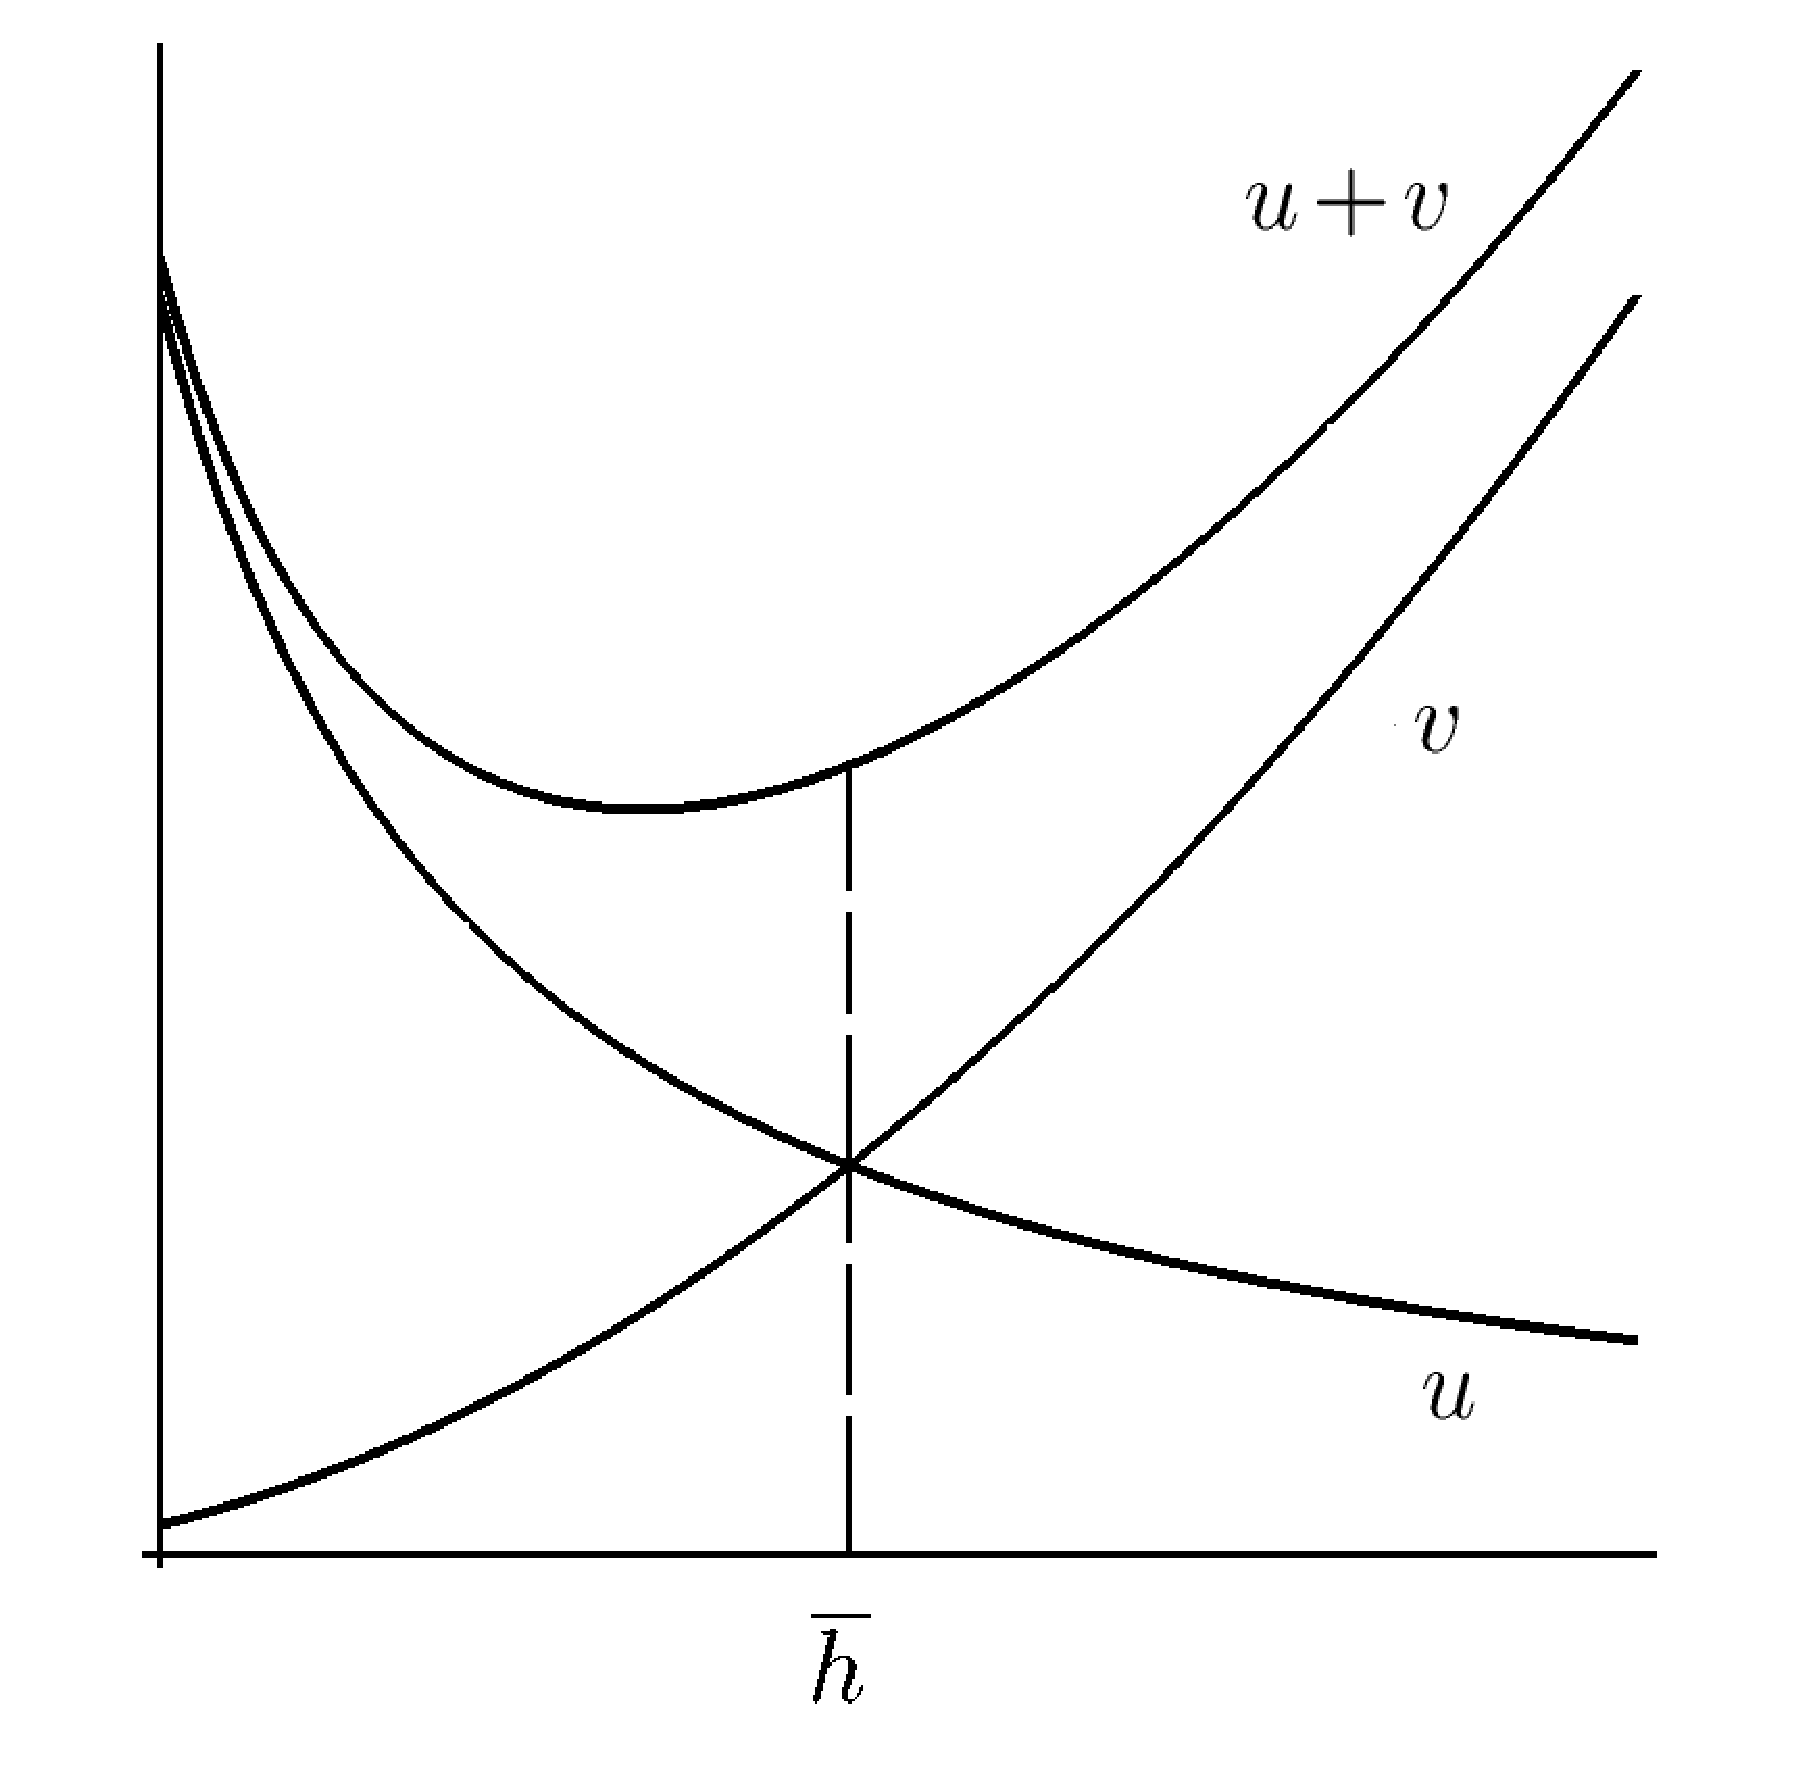
\includegraphics[width=0.4\textwidth]{pict/pict20-1.eps}
\end{center}
 \bigskip
 \refstepcounter{ris}\label{r20-1}

 \centerline{Рис.~\theris}
 \bigskip
\end{figure}


В правой части~(\ref{f20-4}) слагаемое  $h^{-k}$ убывает, а $h^{l-k}$
возрастает; исходя из сформулированного принципа выберем точку
 $h=\overline h$ из
 условия $(\overline h)^{-k}\|f\|_C=(\overline h)^{l-k}\|f^{(l)}\|_C,$ что дает значение
 $$
  \overline h=\left( \frac{\|f\|_C}{\|f^{(l)}\|_C}\right)^{\frac{1}{l}}.
 $$
 Подставив найденное значение $h$
 в~(\ref{f20-4}), получим неравенство Колмогорова
 $$
 \|f^{(k)}\|_C\le {2C_k}\|f\|_C^{\frac{l-k}{l}}\|f^{(l)}\|_C^{\frac{k}{l}}.
 $$
 Теорема доказана с константой, не зависящей от $n:\ K_{n,k}\le \pi A_k.$

 З\,а\,м\,е\,ч\,а\,н\,и\,я.\quad
 1) Неравенство Колмогорова верно   и доказательство проходит
 для любого однородного пространства
 $2\pi$-периодических функций (см. замечание~\ref{r16-1}), так как
 обобщенное неравенство Бернштейна верно для этих
 пространств. В частности, оно справедливо в $L_{2\pi}^p$

 2) Как уже отмечалось в лекции 19, неравенство~(\ref{f20-1}) справедливо и для функций на всей
 числовой прямой.


 Смысл неравенства Колмогорова заключается в
 следующем: если какому-то пространству принадлежит
 функция и ее старшая производная $f^{(l)},$
 то тому же пространству принадлежат и все промежуточные
 производные.

 Неравенство Колмогорова есть решение следующей
  задачи. Пусть  заданы числа $M_l\ge 0$ и $M_0\ge 0.$
 Рассмотрим все $l$ раз дифференцируемые функции $f,$
  у которых
 $$
 \|f\|_C=M_0,\qquad \|f^{(l)}\|_C=M_l.
 $$
 Какова тогда область изменения норм $\|f^{(k)}\|_C$
 и, в частности,  чему равно $M_k=\max\|f^{(k)}\|_C?$
 Эта область описывается неравенством Колмогорова.

 \section{Теорема о почленном дифференцировании\\ функциональных
 последовательностей}

 Рассмотрим задачу. Пусть дана последовательность периодических
 функций $\{f_n\}$ равномерно сходящаяся к функции $f$:~ $f_n\rightrightarrows
 f$ и функции $f_n$ имеют $k$-ую производную.
 При каких условиях предельная функция дифференцируема $k$
 раз и $f_n^{(k)} \rightrightarrows f^{(k)}?$

Предположим, известно, что производные некоторого порядка  $l>k$ членов
последовательности существуют и ограничены некоторой константой:
 $\|f_n^{(l)}\|_C\le {A},\ n\ge 1.$
 Напишем неравенство Колмогорова для разностей $f_n-f_m$:
  $$
 \|f_n^{(k)}-f_m^{(k)}\|_C\le K \|f_n-f_m\|_C^{\frac{k}{l}}\cdot
 (2{A})^{\frac{l-k}{l}};
 $$
 последнее неравенство показывает, что последовательность производных $\{f_n^{(k)}\}$
 является фундаментальной (последовательностью Коши) и, значит,
 равномерно сходится к некоторой функции $\varphi.$
 Но тогда в силу соответствующей теоремы о равномерно сходящихся
 последовательностях дифференцируемых функций можно утверждать,
 что функция $f$ является $k$ раз дифференцируемой и $\varphi=f^{(k)}$.

 Отсюда следует, что на классе  функций, $l$
 раз дифференцируемых, с производной порядка $l,$ ограниченной некоторой константой,
 операция дифференцирования порядка  $k,$~ $0<k<l,$ корректна, а точнее, оператор
 дифференцирования порядка $k$ непрерывен. Это
 означает, что на таком классе имеет место регуляризация оператора
 дифференцирования: малая ошибка в определении функции $f$
 из класса гарантирует малость ошибки вычисления
 производных $f^{(k)}\ (0<k<l)$ при подходящем методе их
 восстановления по $\widetilde{f}(x) (\approx f(x)).$

 Пусть $f\in {C}^{(l)}_{{2\pi}}$ и $t_n$~--
 некоторый тригонометрический полином.
 Применим к разности $f-t_n$ неравенство Колмогорова:
 $$
 \|f^{(k)}-t_n^{(k)}\|_C\le K \|f-t_n\|_C^{\frac{k}{{l}}}\cdot
 \|f^{(l)}-t_n^{(l)}\|_C^{\frac{l-k}{l}}.
 $$
 Отсюда следует, что если функция и  ее старшая производная
 хорошо приближаются тригонометрическим полиномом и его
 {старшей} производной, то и промежуточные производные
 функции тоже хорошо приближаются
 {соответствующими} {производными полинома}.

 Если в качестве $t_n$ возьмем суммы Фурье, то получим оценку
 $$
   \|f^{(k)}-s_n^{(k)}\|_C\le K_{{1}} \|f-s_n \|_C^{\frac{k}{l}}\cdot
   \Big(\ln (n+1)  {E_n(f^{(l)})\Big)^{\frac{l-k}{l}},\qquad n\ge 1},
 $$
 которая дает связь между приближениями производной и функции
 суммами Фурье.

 Отметим, что в неравенстве Колмогорова~(\ref{f20-1}) в пространстве $C_{2\pi}$
 нельзя заменить нормы на наилучшие приближения, так как в
 пространстве $C_{2\pi}$ наилучший полином для производной может не быть
 производной от наилучшего полинома для функции. В $L_2$ такая замена возможна.

Имеется большое число исследований, посвященных более общим
 в сравнении с~(\ref{f20-1}) неравенствам\footnote{Информацию по
 этой тематике можно найти в обзорной работе:
Арестов В.\,В. Приближение неограниченных операторов ограниченными и
родственные экстремальные задачи
 // Успехи матем. наук. 1996. Т.\,51, вып.\,6. С.\,89--124.}
 $$
 \|f^{(k)}\|_{L_q}\le K\|f\|_{L_p}^{\alpha}\cdot
 \|f^{(l)}\|_{L_r}^{\beta}.
 $$


 \section{Неравенство Джексона}

 {Промежуточные приближения (приближения гладкими
 функциями)}
 \vspace{3mm}

 Известно, что всякую непрерывную периодическую  функцию можно сколько угодно
 точно приблизить гладкими функциями. Например, суммами
 Фейера:
 $$
 \forall\ f\in C_{{2\pi}}\qquad \forall\ \varepsilon>0\qquad \exists\ n:\qquad
 \|f-\sigma_n{(f)}\|_C<\varepsilon.
 $$
 Зададим нормировочные параметры. Пусть $l$
 -- натуральное число и $M>0.$ Рассмотрим класс $C^{(l)}(M)$ всех
 $l$ раз непрерывно дифференцируемых $2\pi$-периодических
 функций $\varphi,$ у которых  $\|\varphi^{(l)}\|_C\le M.$
 Классом $C^{(l)}(M)$ ($M$ -- фиксировано) уже нельзя  сколь угодно точно
 приблизить произвольную
 функцию. Возникает следующая проблема.

 \task %%% Задача.
 Найти
 $$
 \inf_{\varphi\in C^{(l)}(M)} \|f-\varphi\|_C=E(f,C^{(l)}(M)).
 $$
 Эта задача бесконечномерная и нелинейная.

\vspace{3mm}
 {\bf 1. О сглаживании функций}
 \vspace{3mm}

 При $l=1,2$ классическое решение задачи о сглаживании дается
 с помощью определяемых ниже функций Стеклова.

 Пусть $h>0;$ усредним функцию $f{\in C_{2\pi}}$ по отрезку
 длины $h$ с центром в точке $x.$  В результате получим функцию
    \begin{equation}\label{f20-VAS-1}
  f_h(x)=\frac{1}{h}
 \int_{-\frac{h}{2}}^{\frac{h}{2}} f(x+t)\, dt,
\end{equation}
 которая называется  функцией Стеклова. Сглаженная функция~(\ref{f20-VAS-1})
 уже непрерывно дифференцируема и
 $$
 f_h'(x)=\frac{1}{h} \left\{ f\left( x+\frac{h}{2}\right)-f\left(
 x-\frac{h}{2}\right)\right\}.
 $$
 Справедливы следующие соотношения:
 $$
 \|f_h'\|_C\le \frac{2}{h}\|f\|_C,
 $$
 $$
 \|f-f_h\|_C\le \frac{1}{h}
 \int_{-\frac{{h}}{2}}^{\frac{{h}}{2}} \| f(x)-f(x+t)\|_C\, dt\le
 \frac{2}{h}
 \int_{0}^{\frac{h}{2}} \omega(f,t)\, dt\le \omega\left(
 f,\frac{h}{2}\right).
 $$
 Следовательно, функция Стеклова приближает исходную функцию и является непрерывно
 дифференцируемой. Однако, при хорошем приближении производная $f'_h,$ вообще говоря,
 будет большой.

 По вещественному числу $M>0$ выберем параметр $h$ так, чтобы $M=\dfrac{2}{h}\|f\|_C,$
 т.\,е. возьмем $h=\dfrac{2\|f\|_C}{M}.$ В результате приходим к следующему утверждению о приближении функциями Стеклова.

 \begin{teo} Для каждой функции $f\in C_{{2\pi}}$ и любой константы $M>0$ существует
 непрерывно дифференцируемая функция $\varphi$ со свойством
 $\|\varphi'\|_C\le M$ такая,~что
 $$
  \|f-\varphi\|_C\le \omega\left( f,\frac{\|f\|_C}{M}\right).
 $$
 \end{teo}

 Аналогично исследуется случай $l=2.$
Рассмотрим вторую разность
   $$
 \Delta_t^2 f(x)=f(x+t)-2f(x)+f(x-t).
 $$
 Проинтегрировав 2 раза, получим соотношение
  \begin{equation}\label{f20-5}
 \frac{1}{h^2}\int_0^{h}\int_0^{t_1} \Delta_t^2 f(x)\, dt\
 dt_1=\varphi(x)-f(x),
 \end{equation}
 в котором
  \begin{equation}\label{f20-5a}
 \varphi(x)=\frac{1}{h^2}\int_0^{h}\int_0^{t_1} (f(x+t)+f(x-t))\, dt\
 dt_1.
  \end{equation}
 Сделав в одном интеграле замену переменного $x+t=u,$ а во втором $x-t=u,$ получаем представление
 $$
 \varphi(x)=\frac{1}{h^2}\int_0^{h}\int_{x-t_1}^{x+t_1} f(u)\ du\  dt_1.
 $$
 Эта функция дифференцируема по $x$ и
 $$
 \varphi'(x)=\frac{1}{h^2}\int_0^{h}(f(x+t_1)-f(x-t_1))\  dt_1=\frac{1}{h^2}\left(\int_x^{x+h}f(v)\ dv-\int_{x-h}^{x}f(v)\ dv\right).
 $$
Последнее выражение вновь дифференцируемо, а, значит, функция $\varphi$ дважды
дифференцируема и
 \begin{equation}\label{f20-6}
 \varphi''(x)=\frac{1}{h^2}\left(f(x+h)-2f(x)+f(x-h)\right).
\end{equation}

Следовательно, функция $\varphi$ дважды непрерывно дифференцируема и, как нетрудно
увидеть из~(\ref{f20-6}) и~(\ref{f20-5}), обладает следующими свойствами:
 \begin{equation}\label{f20-7}
 \|\varphi''\|_C\le \frac{1}{h^2} \|\Delta_h^2 f\|_C\le\frac{4}{h^2}\,\|f\|_C,\qquad
 \|f-\varphi\|_C\le \frac{1}{2}\,\omega_2(h,f).
 \end{equation}

 \vspace{3mm}
 {\bf 2. Неравенство Джексона в ${C_{2\pi}}$}
 \vspace{3mm}

 Процедура сглаживания  и неравенство Фавара позволяют
 оценить приближение произвольной функции через характеристики ее гладкости.

 \begin{teo}[Д.\,Джексон]
 При любом $k\ge 0$ существует константа $C_k$ такая, что для функций
 $f\in {C}^{(k)}$ справедливо неравенство
  $$
 E_n(f)_C\le \frac{C_k}{(n+1)^k}\, \omega_2\left(
 \frac{1}{n},f^{(k)}\right).
 $$
 \end{teo}

 \begin{proof} %%% Доказательство.
 По неравенству Фавара~(\ref{f19-5})
 $$
 E_n(f)_C\le \frac{M_k}{(n+1)^k} E_n(f^{(k)})_C;
 $$
 теперь достаточно оценить $E_n(f^{(k)})_C.$ Построим  функцию   $\varphi$  (см.~(\ref{f20-5a}))
 для производной $f^{(k)}$ со значением параметра  $h=\dfrac{1}{n}.$
 Тогда  в силу~(\ref{f20-7}) будем иметь
 $$
 \|\varphi''\|_C\le  n^2
 \left\| \Delta_{\frac{1}{n}}^2 f^{(k)}\right\|_C\le
  n^2\omega_2\left( \frac{1}{n},f^{(k)}\right)
 $$
 и, следовательно, по неравенству Фавара
 $$
 E_n(\varphi)_C\le \frac{M_2}{(n+1)^2} n^2\omega_2
 \left( \frac{1}{n},f^{(k)}\right).
 $$
 Поскольку
 $$
 E_n(f^{(k)})_C\le E_n(f^{(k)}-\varphi)_C+E_n(\varphi)_C\le \|f^{(k)}-\varphi\|_C+E_n(\varphi)_C,
 $$
 то (вновь с помощью~(\ref{f20-7})) приходим к оценке
  $$
 E_n(f^{(k)})_C\le \left(\frac{1}{2}+M_2\right) \omega_2
 \left( \frac{1}{n},f^{(k)}\right).
 $$
 Теорема доказана.
 \end{proof}

 При $k=0$ получаем   неравенство Джексона для недифференцируемых функций
 $$
 E_n(f)_C\le C\omega_2\left( \frac{1}{n},f\right).
 $$

 \begin{Remark} %%% Замечание.
 Это доказательство теоремы Джексона проходит в любом однородном пространстве.
 \end{Remark}
